\chapter{Data Analysis}
In this chapter we will present how the simulation is run and how the results are analyzed.

\section{Running the simulation}

In order to run a simulation three parts are needed:

\begin{itemize}
    \item \textbf{simulation software:} Which is a binary file of the simulation software available for Mac/Win/Linux
    \item \textbf{Simulation Parameters:} A JSON text file that defines Simulation Parameters
    \item \textbf{Classroom Profile:} A JSON text file that specifies the psychological profiles of students in the class
\end{itemize}

The simulation can be run interactively making it possible to observe the progression
of the simulation, or in headless mode, where no visualization is generated.
The later one is particularly useful in combination with a increased simulation
speed. The combination of a headless mode with increased simulation speed can be
used to run many different simulations in a \textbf{batch mode} like manner.

\bb

Independent of the way the simulation is run, it will generate a CSV file that
documents the progress of the simulation. That CSV file can be opened in any
arbitrary tabular data processing software (e.g Excel) for manual inspection, but
is made to be analyzed by a set of python scripts developed for the purpose.

How those scripts are used and what results they generate is described in the following chapters.

\section{Data Analysis Pipeline}
The Data Analysis performed for the complete thesis is split into three parts, each 
having a distinct focus, answering a different set of questions.

\begin{enumerate}
    \item \textbf{Simulation:} The goal of the simulation is to study the behavior
    of a particular classroom, ranging from the behavior of a single agent to the
    aggregated and average behavior of group as a whole.
    \item \textbf{Experiment:} How much variation is there between multiple runs of
    the simulation for the same classroom, slightly changing the classroom profiles and
    random elements of the simulation?
    \item \textbf{Study:} Having a expectation on how a specific classroom profile
    behaves, how two different profiles compare to each other, and how alterations
    of the personality profile effect group averages?
\end{enumerate}

In the following chapters we will have a look at each step of the pipeline individually,
as it is not necessary to always run the complete pipeline but based on the question
one tries to answer only one or two of the first steps.

\section{Simulation}
\begin{figure}[!h]
    \hspace*{-2.0\leftmargin}
    \makebox[\textwidth][l]{%
    \begin{minipage}[t]{10cm}
        \centering
        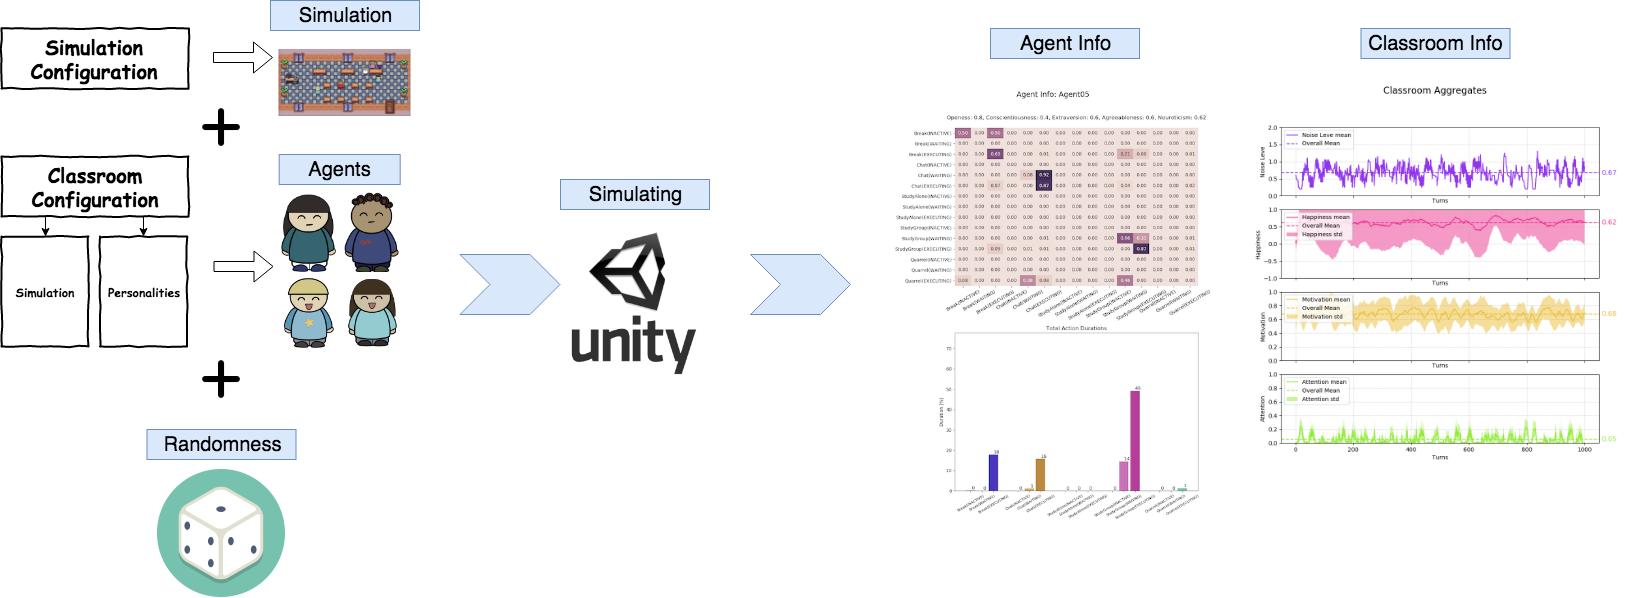
\includegraphics[width=500pt]{Simulation-Overview}
        \caption{Simulation Overview}
        \label{SimulationOverview}
    \end{minipage}    
    }%
\end{figure}

Simulation is the first step of the analysis, answering the question how a specific
classroom of agents behaves.

The input to the simulation are three things. The simulation config, defining
all simulation relevant constants that governing how the simulation mechanisms,
the classroom configuration that defines the psychological profile of students,
and a random seed that is used to initialize the random number generator used during
the simulation.

Examples of the simulation config and classroom config can be found as part of
the appendix (see \ref{ApxSimulationConfig} abd \ref{ApxClassroomProfile}).

The classroom configuration must contain a set of Personality Types and the number
of students of each type. When the simulation is run, a classroom is dynamically
generated with agents following the in the classroom configuration defined composition
of profiles.

The python analysis scripts for the simulation will read the CSV file generated
after the simulation is complete and generate a set of figures containing information
about each individual agent, the classroom as a group and a new CSV file that contains
aggregated information.

\subsubsection{Agent Info}
The analysis result specific to each agent is a \textbf{Agent Info} figure (see \ref{AgentInfo} showing
three different figures) that contains information about the distribution and transitions
between different behaviors performed by the agent. This figure is used to study how
a specific instance of a psychological type behaves in the given classroom.
One can observe how much of the overall time an Agent spends Studying alone or example
and how long on average a single study session lasts.

It is interesting to observe how different the different Traits of the Big-Five
effect the behavior distribution of the individual agent. So could one observe that
agents high on conscientiousness for example on average have longer learning sessions
that agents with a low level of conscientiousness.

\begin{figure}[H]
    \label{AgentInfo}
    \hspace*{-2.0\leftmargin}
    \makebox[\paperwidth][l]{%
        \begin{minipage}[t]{180pt}
            \centering
            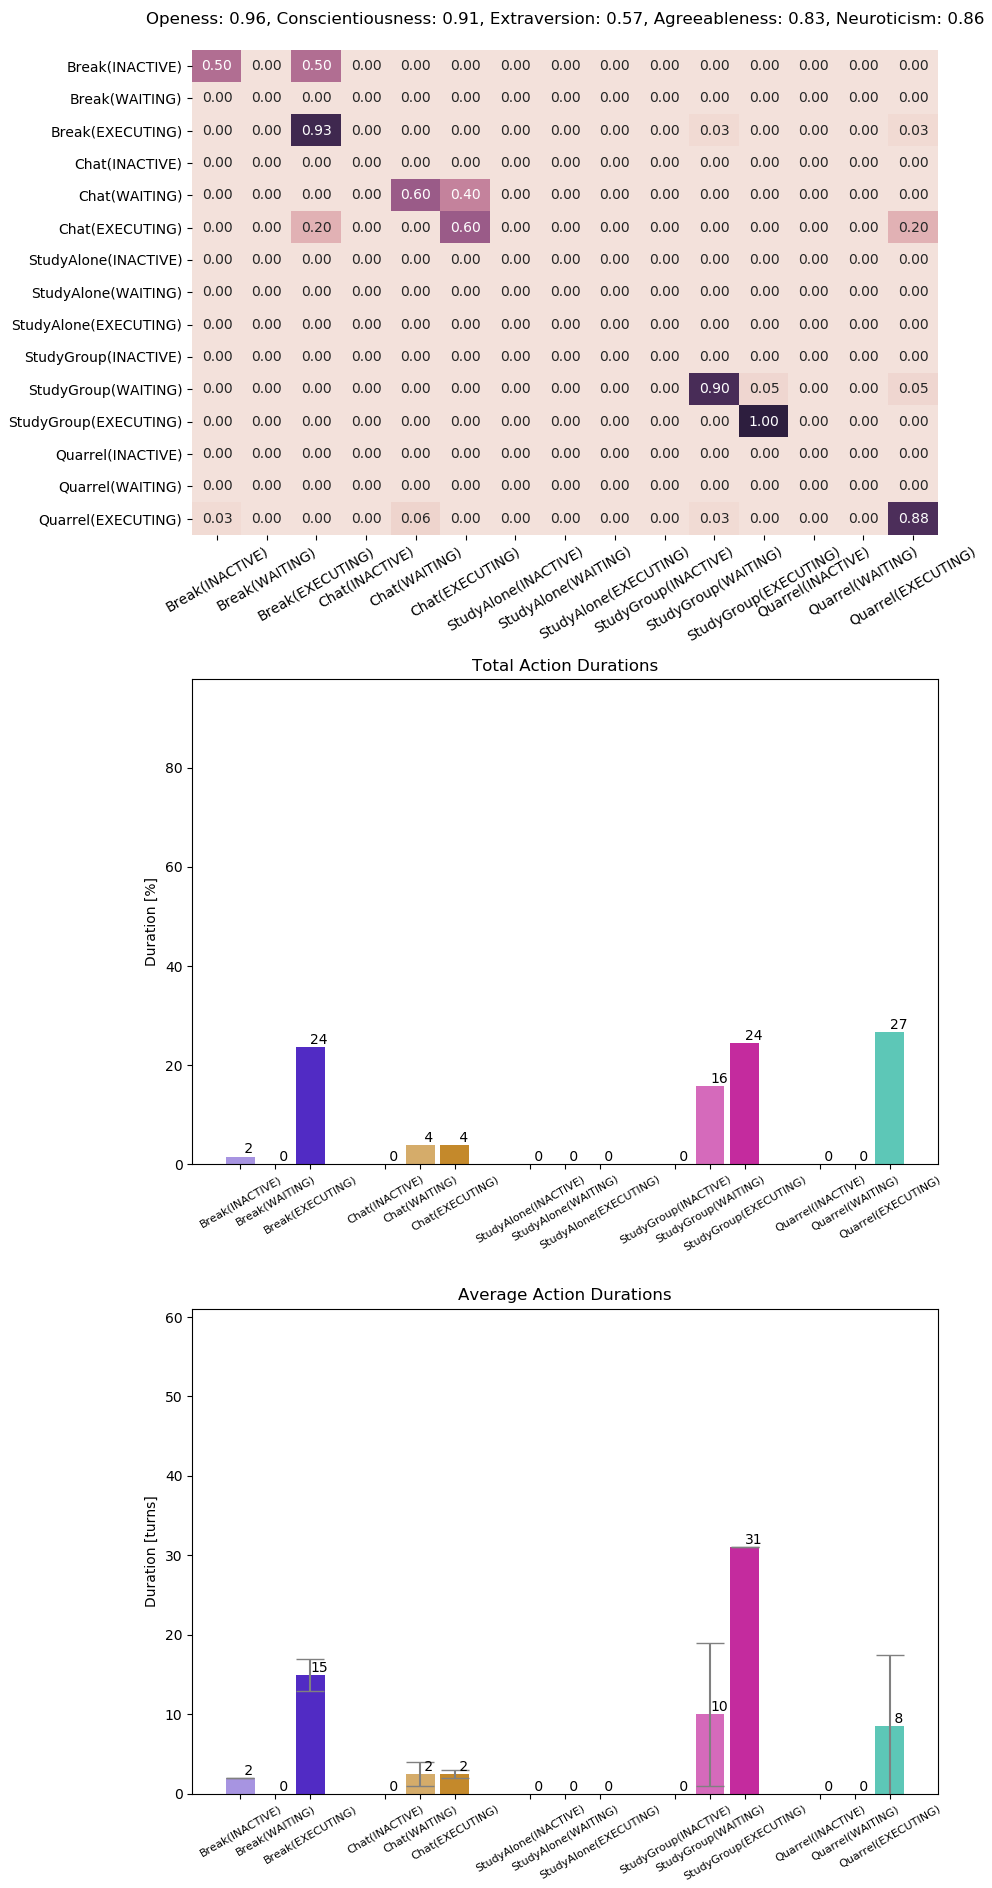
\includegraphics[width=170pt]{AgentInfo1}
            \caption{Agent Info #1}
        \end{minipage}
        %\hspace{3cm}
        \begin{minipage}[t]{180pt}
            \centering
            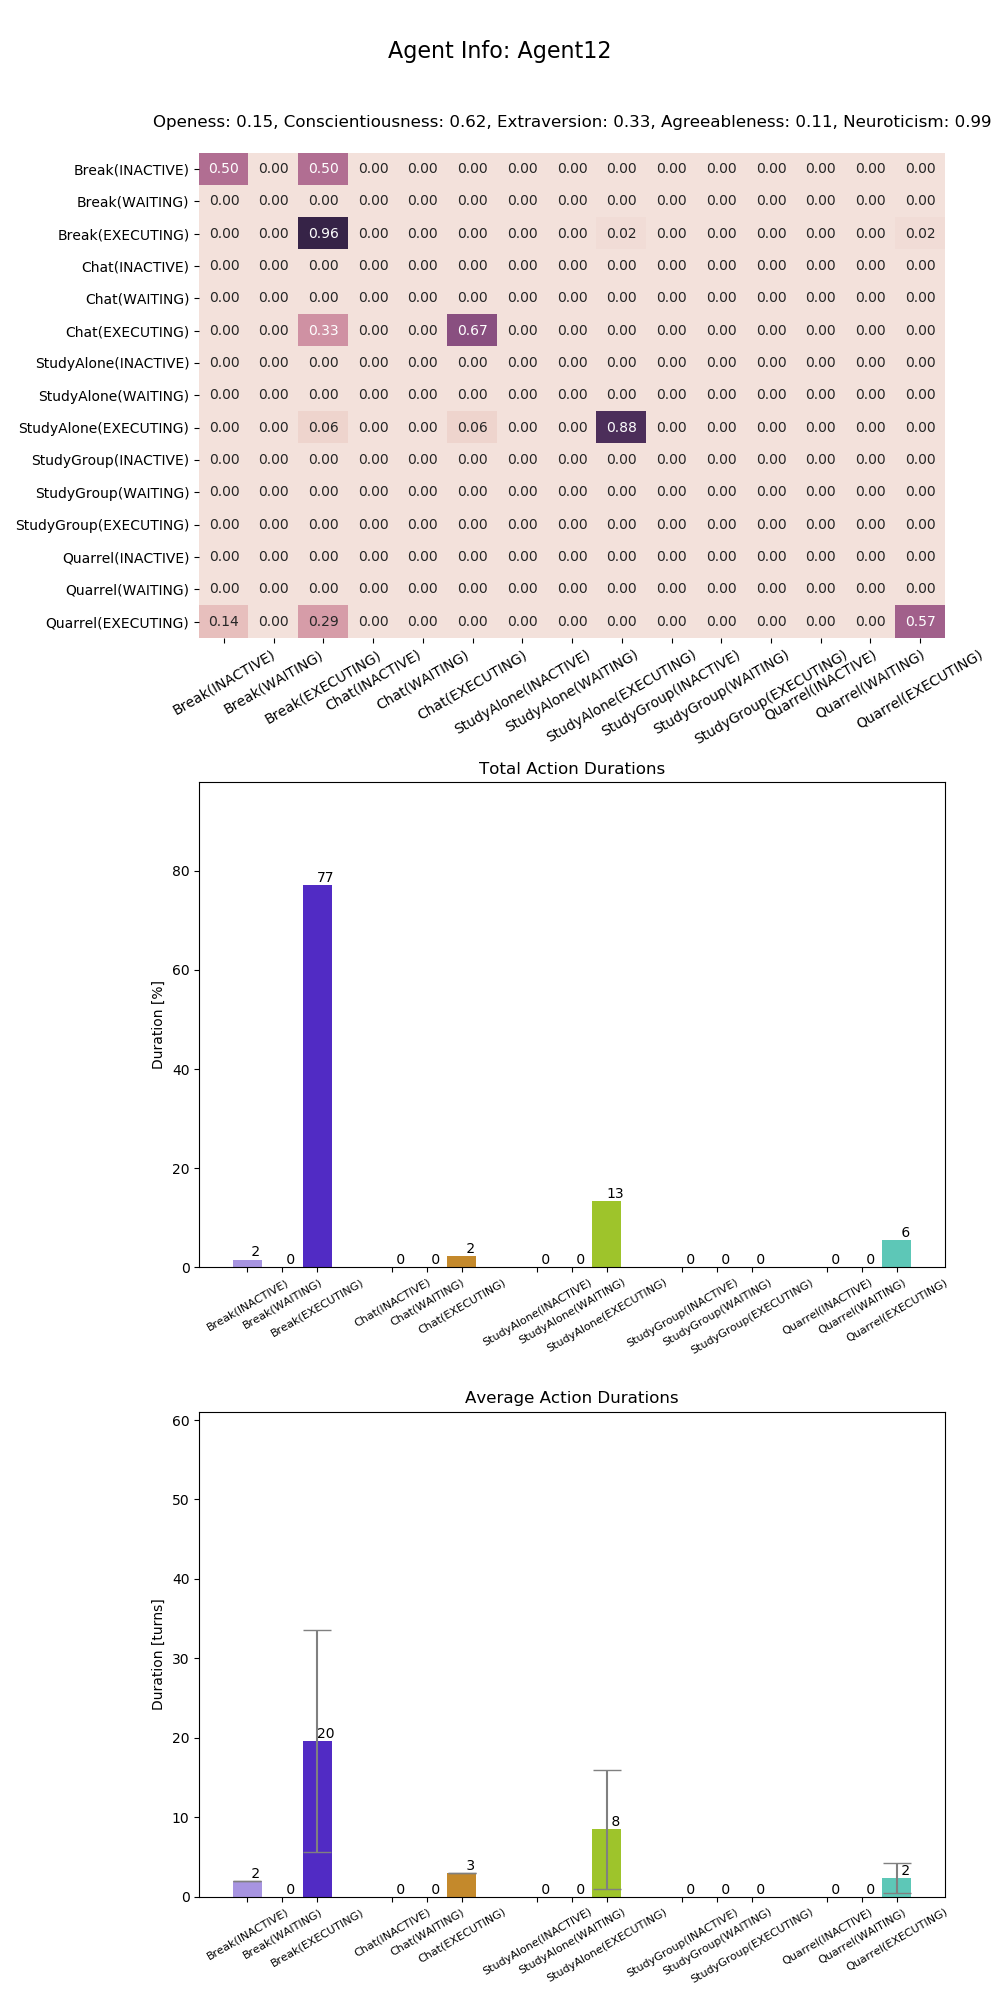
\includegraphics[width=170pt]{AgentInfo2}
            \caption{Agent Info #2}
        \end{minipage}
        \begin{minipage}[t]{180pt}
            \centering
            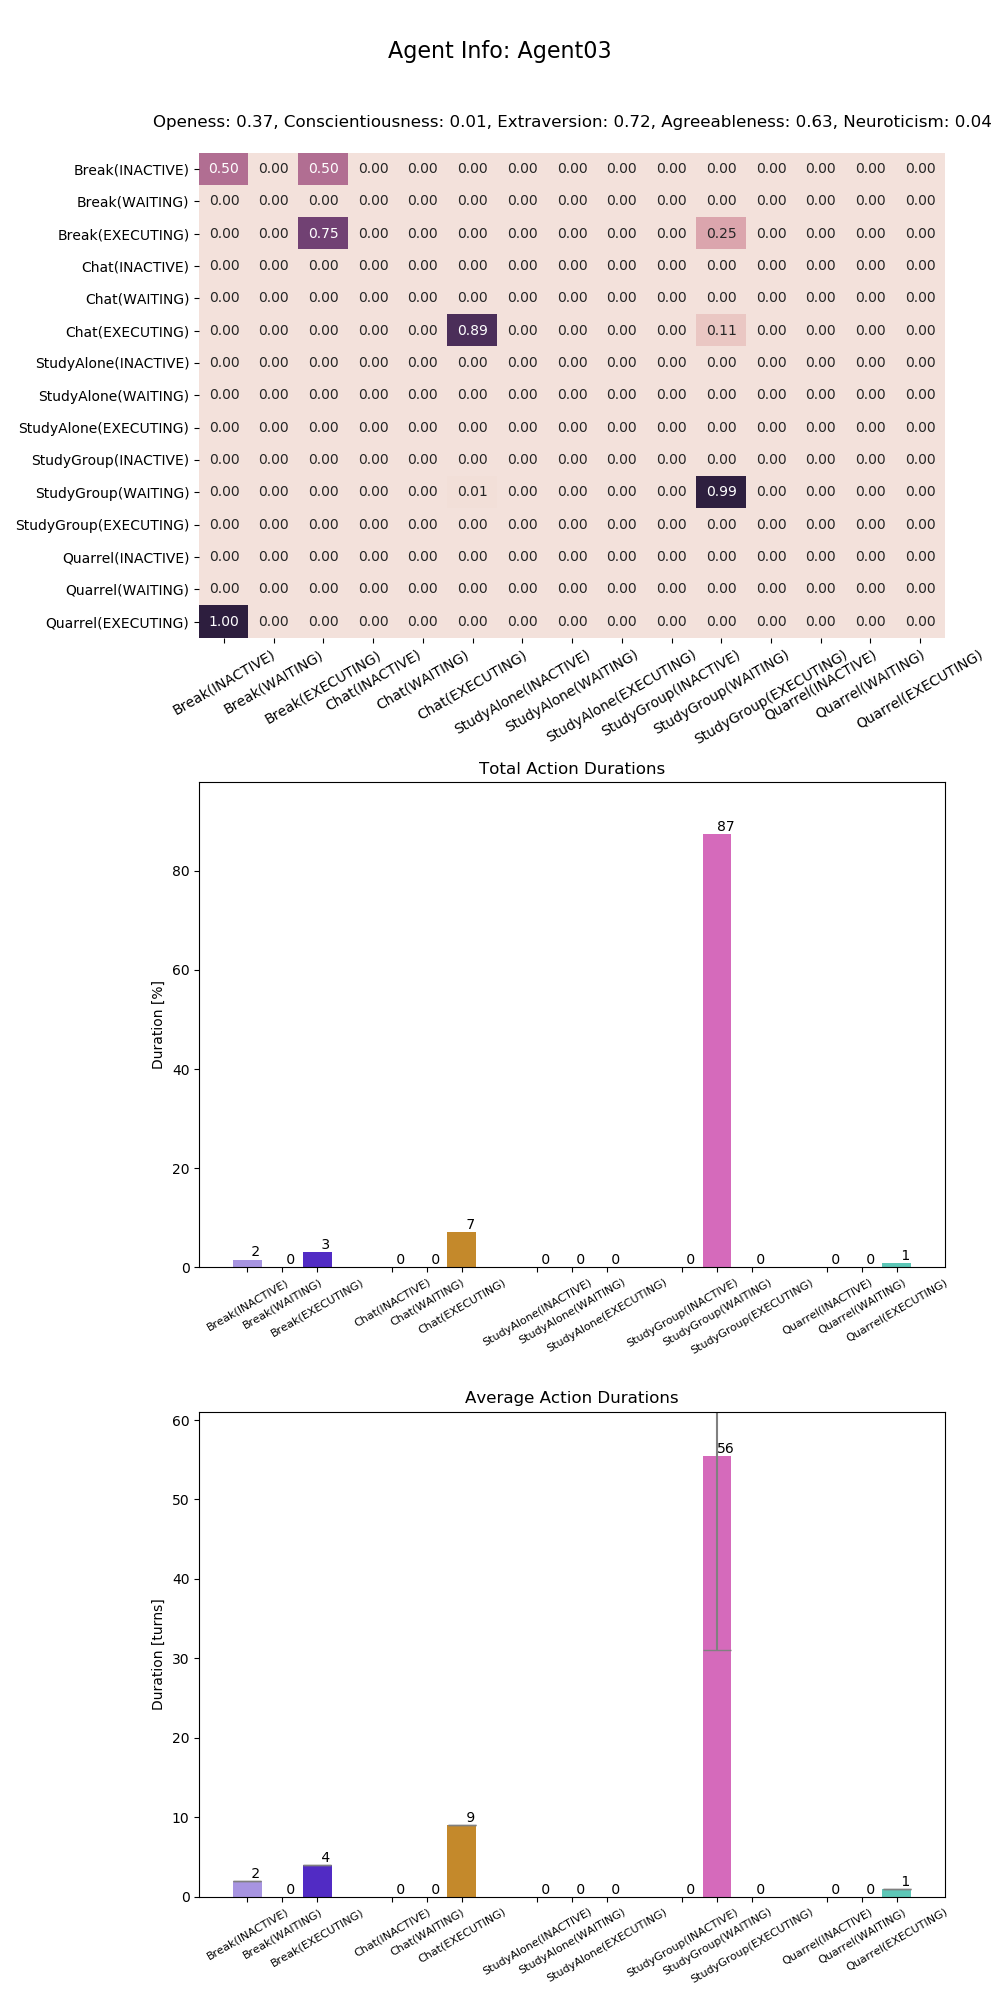
\includegraphics[width=170pt]{AgentInfo3}
            \caption{Agent Info #3}
        \end{minipage}
    }%
\end{figure}

\subsubsection{Classroom Aggregates}
The second result of the simulation analysis is a figure showing classroom
aggregated features over time (see figure \ref{ClassroomAggregates} as an example).
This figures contains information like the aggregated noise, the average happiness,
motivation and attention of a class, in addition to information about how many of
the students are studying or quarreling at a specific moment during the simulation.

\begin{figure}[H]
    \makebox[\textwidth][l]{%
    \begin{minipage}[t]{10cm}
        \centering
        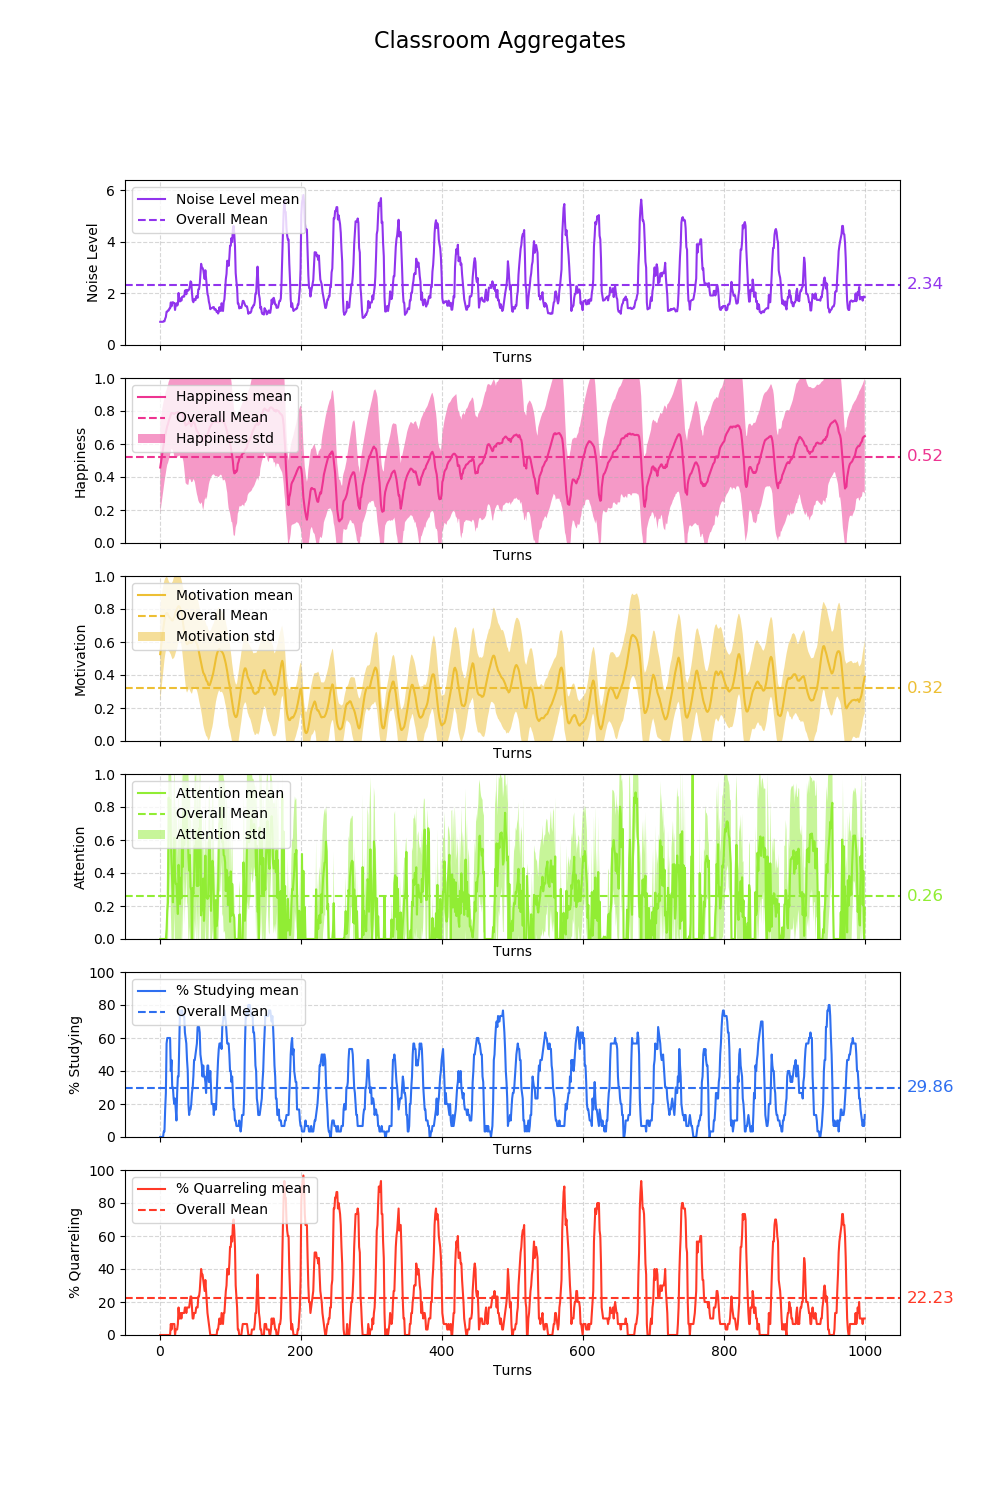
\includegraphics[width=400pt]{ClassroomAggregates}
        \caption{Classroom Aggregates}
        \label{ClassroomAggregates}
    \end{minipage}    
    }%
\end{figure}



\section{Experiment}
The experiment is the second phase of the data analysis pipeline and is focused
on evaluating the variance between simulations of the same classroom configuration.

\begin{figure}[H]
    \makebox[\textwidth][l]{%
    \begin{minipage}[t]{10cm}
        \centering
        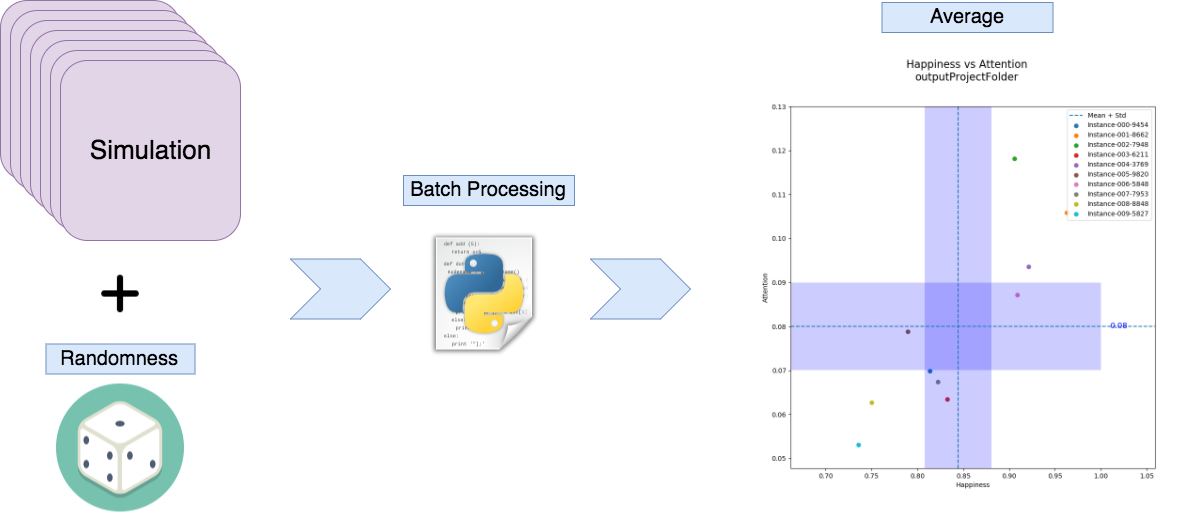
\includegraphics[width=400pt]{Experiment-Overview}
        \caption{Experiment Overview}
        \label{ExperimentOverview}
    \end{minipage}    
    }%
\end{figure}


This is achieved by running multiple instances of the same simulation (identical simulation 
and classroom configs) but different seed values for the random number generator used
during the simulation.

Depending on the classroom configuration, agent personality can be partially random,
and the actions selection has a random element, and interactions are effected by
the random number generator.

The results of the experiment phase is a single \textbf{HA-Plot} plot named after
its axis Attention vs. Happiness. The plot shows a point for each simulation instance based on
the average attention and happiness of the classroom over the complete simulation.
In addition the overall happiness and attention average for all instances is
indicated with two solid lines, and the corresponding standard deviation with
semi transparent bars.

The plot visualizes the spread between different instances of the simulation, and
could be used to detect outliers and estimate the stability of a specific classroom
configuration.

In addition to the HA-Plot a CSV file is generated that contains the average
happiness and attention values for each agent and classroom for all simulation instances.
This dataset basically is the numeric equivalent to the generated HA-Plot.

\section{Study}
The last step in the data analysis pipeline is focused on comparing different classroom
profiles.

\begin{figure}[H]
    \makebox[\textwidth][l]{%
    \begin{minipage}[t]{10cm}
        \centering
        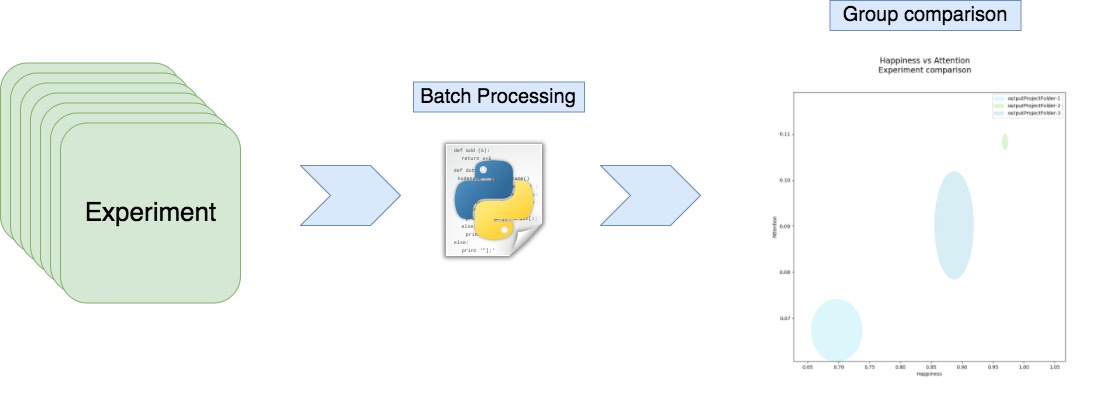
\includegraphics[width=400pt]{Study-Overview}
        \caption{Study Overview}
        \label{StudyOverview}
    \end{minipage}    
    }%
\end{figure}

In the last step the CSV generated during the Experiment phase is anlayzed to
generate a HA-Plot that contains one ellipse for each classroom profile simulated.
The center of the ellipse are put to the overall mean attention and happiness
of for the set of instances of the same classroom profile, indicating its standard
deviation by the shape of the ellipse.
